%\chapter{概要}

\begin{abstract}
本稿では,類似画像検索技術とテキスト検索を用いた自動画像アノテーションについて述べる.
提案手法は,大きく二段階に分けられる.
一段階目では,Web上からクエリで指定した物体の周辺テキスト付き画像を収集する.
二段階目では,収集した画像がクエリで指定した物体を表しているかどうかの分類を,
画像特徴量を用いた類似画像検索と周辺テキストを用いたテキスト検索の二手法を用いて行う.
この際,テキスト検索の結果を加味した分類結果としなかった場合の分類結果を比較することで,
自動画像アノテーションにおける日本語テキストの有用性を示した.
\end{abstract}
%\thispagestyle{empty}


%\setcounter{page}{1}

\chapter{はじめに}



近年,非常に多くの画像がWeb上にアップロードされている.
Web上の画像は多くの場合周辺テキストを伴っている.
これら非常に多くの周辺テキストを伴った画像を利用しようする試みの一つとして画像アノテーションがある.
画像アノテーションは画像が表す内容に対応するメタデータを付与する技術であり,近年活発に研究がなされている\cite{jeon,watanabe}.

画像アノテーションは一般物体認識の要素課題の1つでもある.
% 計算機で検索できるようにしようとする試みが行われている.
% しかし,計算機が多様な画像データの内容を理解するのは困難である.
% そこで計算機が自動で画像を理解するための一般物体認識と呼ばれる技術が求められている\cite{yanai}.
一般物体認識とは,制約のない画像中の物体を検出,認識して
その認識対象の一般的な名称を出力する技術である.
例えば「自転車」が中央に表示されている画像を入力すると「自転車」というテキストが出力がされるようなシステムが一般物体認識である.
一般物体認識は画像認識の研究において最も困難な課題の一つとされている.
%ここで一般物体認識の参考文献をなにかcite
%可能ならここに色ヒストグラムを使った画像認識技術の話題を追加
%画像アノテーションはこの一般物体認識の要素課題の1つである.
%画像アノテーションは画像が表す内容に対応するメタデータを付与する技術であり,近年活発に研究がなされている\cite{jeon,watanabe}.
%
本研究では,この様な画像認識の問題として
トレイニングデータを自動生成する課題に注目する.
例えば次のような場合に注目する:
%\begin{itemize}
%\item 
今まで雑種として扱われていた猫の中で尻尾の丸い猫が日本猫として雑種とは別に扱うようになった.
日本猫を画像認識するためのトレイニングデータとして画像を数百枚収集せよ.
%\end{itemize}



画像アノテーションの先駆けとなった研究として森ら\cite{mori}は,百科事典中の画像と説明文から,
画像の部分的な領域と単語の対応を学習することで,
未知の画像から関連する単語を出力する手法を2001年に提案した.
しかし,当時の環境では膨大な認識対象の物体に対して十分なデータ量を用意出来なかったため,認識精度は限定的なものであった.

しかし今日ではインターネットの発展を背景とした,Web上の画像を用いた画像アノテーションの研究が発展している.
例えばImageNet\cite{imagenet}は,WordNetのオントロジーを利用して,その単語の表す物体の画像を人手で収集したデータベースであり,
2012年2月の時点で21,841 の概念,14,197,122 の画像が利用可能である.
ImageNetは人手で画像を分類しているため,誤分類が少なく,機械学習を用いた画像分類の実験によく用いられている. 

これに対して,画素数が少なく画質も悪い画像を大量に収集し,
それらを直接使うことによって画像アノテーション認識を行う事例ベースの手法が提案されている.
例えば,Torralba\cite{torralba}らは,Web検索エンジンを用いて75,062カテゴリ,
約8,000 万枚の画像を収集したTinyImagesと呼ばれるデータベースを用い,
単純な画像特徴量による{\it k}近傍探索を行うことにより,画像アノテーションが可能であることを示した.

本稿では,類似画像検索とテキスト検索を用いた画像アノテーションを用る.
提案手法として,まずWebから物体名をクエリに指定し検索を行い,得られた画像と周辺テキストを収集し,
収集した画像がクエリで指定した物体を表しているかどうかの分類を画像特徴量を用いて行う.
この時,周辺テキストを用いたテキスト検索による上記の分類も行い,
その結果を利用した場合の分類結果としなかった場合の分類結果を比較することで,
自動画像アノテーションにおける日本語テキストの有用性を示す.


%%???
本稿は以下の構成をとる.
\ref{sec:related}節で画像アノテーションの関連研究を紹介し,
\ref{sec:method}節で自動画像アノテーションの問題定義と説明を行う.
4節で提案手法について説明する.
5節では提案手法を用いた実験の結果および評価について述べる.
最後に6節でまとめる.

\chapter{関連研究}
\label{sec:related}

\section{画像認識}

近年,画像認識や画像検出を使った多くの応用が行われている.
この画像検出手法として最も利用されているアルゴリズムがBoosted Cascade\cite{Viola01rapidobject}である.
Boosted Cascadeは家庭用のパソコン程度の処理能力で人間の顔の様な複雑な画像をリアルタイムで検出することができる.
また専門家がパラメータチューンする必要もほとんどない.
これが多くの応用で利用されている理由である.
必要とする学習画像は,達成したい精度にもよるが,
顔検出を行う場合には顔の画像が5,000枚,顔以外の画像を3,000枚程度使った場合に90\%程度の検出率を達成することができる
\cite{Lienhart03empiricalanalysis}
.
顔以外の対象,例えば犬,柴犬,猫,ペルシャ猫といった対象をある程度以上の精度で画像検出するにも
学習画像に5,000枚程度の検出対象の画像が必要となることが予測できる.
多くの場合は
ImageNet\cite{imagenet}
の分類済みの画像を利用することができる.
しかしImageNetに存在しない画像,例えば発売されたばかりの新製品や新種の動物などを画像検出するには
人手で5,000枚の学習画像を用意する必要がある.
この作業をWebマイニングの技術を使って自動化するのが本研究の目的である.

類似画像を利用することで学習画像を減らすこともできる.
Mirrashed\cite{Mirrashed_2013_ICCV}らは
スターウォーズのエイリアンの顔画像800枚から
高精度のエイリアンの顔画像検出器を学習させることに成功している.
これはエイリアンの顔画像と類似した
普通の人間の顔画像を学習に利用することで実現している.
本研究では
精度よりも
自動処理で手間を減らすことを主目的とし,
100枚程度の学習画像を自動収集する方法について検討する.

なんらかのプログラムで自動で収集した画像が全て正しい画像のみであることは稀である.
PaisitkriangkraiらはBoosted Cascadeの学習画像に間違いがどの程度までなら含まれても良いかを調査した
\cite{DBLP:journals/corr/abs-1009-5758}
.
Paisitkriangkraiらは学習画像を変形させノイズを負荷すると検出精度が5%ほど減少することを実験的に示した.
この研究は学習画像に間違いが含まれる割合についての調査ではないが,多少の間違いなら
画像検出器の精度を大幅には落とさないことを示している.
本研究では3割程度までの間違いまでなら許容することとする.
これはBoosted CascadeがBoostingのアルゴリズムに基づいており,
Boostingは自動的に学習データの間違いを除外する性質があることを考えると妥当な値である.



\section{テキスト処理}

Web上の周辺テキストを伴った画像から画像の内容を推定するのが画像アノテーションである.
画像アノテーションの研究は多く存在する.
しかしテキスト処理として英語のテキスト処理を行うものが大部分である.
日本語の周辺テキストを処理する先行研究は発見することが出来なかった.
本研究では日本語テキスト処理を使った画像アノテーションの研究を行う.
%
ここでは
画像アノテーションを行うために
英語のテキスト処理と日本語のテキスト処理でどのような差があるのか
関連研究から類推する.

テキストの中の特定の対象を分類する様な問題の1つとしてposタガーがある.
英語の実用されているposタガーの性能は約8割程度の精度であることが報告されている\cite{BirdKleinLoper09,Ibanez:2011:EPS:1964799.1964819}.
日本語の実用されているposタガーの性能は約9割程度の精度であることが報告されている\cite{UniDicJp2010}.
日本語処理の方が精度が高いことから周辺テキストが日本語の場合の方が高い精度を実現できる可能性がある.
またposタガーとは単語の並んだ順番を処理する技法でもある.
このことから日本語の適当な手がかり表現を利用する手法が高い精度を達成できる可能性が予想できる.


%\chapter{自動画像アノテーション}
%\label{sec:method}
\section{画像アノテーション}
画像アノテーションとは一般物体認識の要素課題の一つであり,
入力された画像が表す内容に対応するメタデータを付与する技術である.


%%%%%%%%%
ここ以後はまだ編集中
%%%%%%%%%


本研究ではその中でも,予め画像と対応するメタデータを学習をしておくことで,
入力画像に自動でメタデータを付与する自動画像アノテーションを行う.
以下ではこのメタデータをラベルと呼ぶこととする.

\section{一般的な手法}
一般的な自動画像アノテーションの概要を図\ref{fig:abst}に示す.

\begin{figure}[tb]
 \begin{center}
  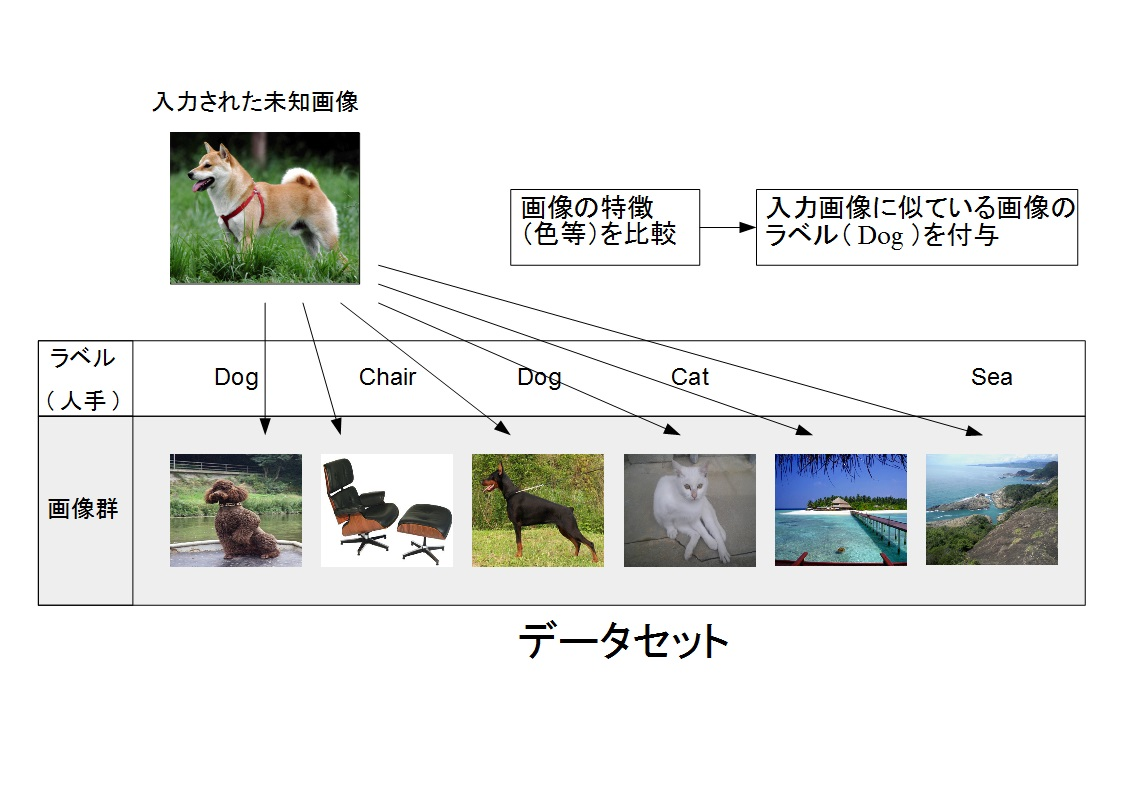
\includegraphics[scale=0.50]{gaiyou.jpg}
 \end{center}
 \caption{一般的な画像アノテーション手法の概要}
 \label{fig:abst}
\end{figure}

まず第一段階として,画像を収集してデータセットを構築し,各画像に人手でラベルをつける.
それらラベルを付けた画像の特徴を統計的に分析することで,ラベルの持つ特徴を学習する.
次に第二段階として,未知の画像を入力し,その画像特徴と類似する画像群が共通して持つラベルを見つけ,
入力画像にそのラベルを付与する.

本稿では,画像の分類手法に工夫をこらし,入力画像に対するラベル付与の精度を高めるための実験を行った.
自動画像アノテーションの分野における主な研究としてはこの他にも,
画像の収集や画像に対するラベル付与を自動化することで,データセットの構築にかける時間と労力を減らす手法などが提案されている.


\section{画像アノテーション}



%前節でラベル付与の自動化・高精度化の手法が研究されていると述べた.
それらの研究の中でも近年頻繁に研究されているものが,画像のブロブ化である.
ブロブ化は各画像を複数の領域に分割し,隣接する領域との特徴の差異を見ることで画像全体を分解することで行う.
これによって得られたブロブは,画像に写っている物体ごとに分割されている可能性が高いので,
注目しているブロブ以外の物体の有無に左右されることなく,そのブロブに対する精確なラベル付与が可能となる.
このブロブ化をデータセット内の全ての画像に施すことで,高精度の画像アノテーションを実現する.

Duygulu\cite{duygulu}らやJeon\cite{jeon}らは,すべての画像はブロブ(画像内の物体の塊)に単語を割り当てることで
内容物を記述することができるという前提で研究を行った.
JeonはDuyguluらの研究を元に,まずブロブと単語の同時分布を予習するためにCMRM(Cross-Media Relevance Model)を開発し,
更にそのモデルを改良した3つのモデルを開発した.
これらは画像を収集する際に自動で画像アノテーションを行う確率的生成モデルである.
その結果,Duyguluらが論文で公開した確率的生成モデルの画像アノテーションの平均精度0.20に比べ,
ほぼ倍の0.41という平均精度を示し,再現率についてもはるかによい結果となった.

またこれらの研究とは別のアプローチで画像アノテーションの精度向上を目指した研究がある.
渡邉ら\cite{watanabe}は,大規模Web画像データベースと
類似画像検索技術を用いた自動画像アノテーションシステムを実装した.
このシステムは,与えられた画像をクエリとして類似画像検索を行い,
検索結果の画像に付随するテキスト中の単語を確率的指標により評価することで,
特別な事前学習なしに画像を意味付けるキーワードを推定可能であることを示した.
このシステムを用いて5カテゴリ30概念の画像に対するアノテーションを行った結果,
10位内正解率がカテゴリ平均で43~75\%,全概念の平均で約59.1\%であった.



%\chapter{類似画像検索とテキスト検索を用いた自動画像アノテーション}
\chapter{提案手法}
\label{sec:way}
\section{概要}
ここでは本研究で提案する自動画像アノテーション手法を説明する.
図\ref{fig:way}に提案手法の概要を示す.
%
\begin{figure}[tb]
 \begin{center}
  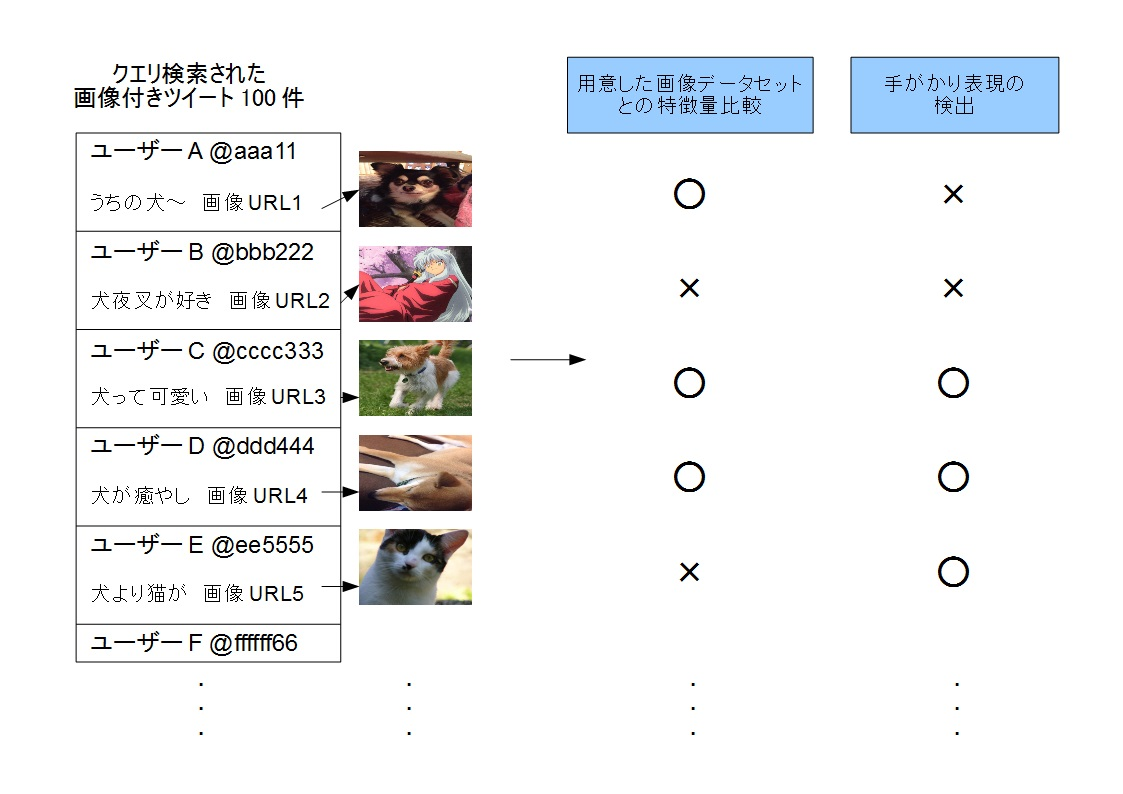
\includegraphics[scale=0.50]{way.jpg}
 \end{center}
 \caption{提案手法の概要}
 \label{fig:way}
\end{figure}
%
提案手法は,Webから得られた画像と周辺テキストを収集する前処理と,
類似画像検索とテキスト検索を用いて得られた画像を分類する処理に分けられる.

前処理においては,TwitterAPIを利用し,認識したい物体名をクエリに指定して検索を行い,得られたツイートを収集する.
収集したツイートから上位100件を選び,それらのツイートに付随するURLからTwitterの公式アップローダにアップロードされた画像をそれぞれ取得する.
%\item 収集したツイートから上位100件を選び,クエリで指定した物体を表しているかどうかを人手で判別する.

画像分類処理においては,まず,ユーザが前処理でクエリとして選んだ物体を表す参考画像を数枚収集し,
その画像を一枚ずつクエリとして,100枚の画像に対して類似画像検索を行う.
参考画像とは,クエリを正しく表していると実験者が判断し,類似画像検索の比較元とする画像である.
類似画像検索は,画像の持つ色や形状などの特徴による検索であり,
この結果,参考画像と見た目の類似した画像が得られる.

また,収集したツイート本文にも手がかり表現を用いてテキスト検索を行う.
この手がかり表現とは,付随する画像が何を表しているかの手がかりとなる表現のことで,
ツイート中からその表現を検索することで,そのツイートに付随する画像がクエリを正しく表現しているか否かの分類が行える.

この二手法を組み合わせ,クエリ単体の自動画像アノテーションを実現している.

以下では,ツイート収集と,類似画像検索,テキスト検索について詳細に説明する.

\section{ツイートの収集}
TwitterAPI1.1の機能を使い,検索したい画像の名称をクエリとし,Twitterからツイートを検索する.
この際,オプションとして" -RT filter:images"をクエリに含めることで,ある程度収集するツイートを選別する.
" -RT"は重複したツイートを取得することを避けるために,
" filter:images"はTwitterの公式アップローダにアップロードされた画像のみを参照するために使用する.

\section{類似画像検索}
本手法では,各色が画像中に何ピクセルあるかを数えた色ヒストグラムを特徴量として比較を行い,
その結果から類似画像の検索を行う.
%OpenCVの色ヒストグラム類似度計測関数のドキュメントに色ヒストグラムを使う手法の詳細や参考文献が書いてあったはずなので色ヒストグラム処理の話を追加してください

そのため,収集したツイートのクエリを正しく表している参考画像を,ツイートに付随する画像とは別に10枚収集する.

まず,収集した画像110枚を全てJPEG形式に変換する.
これは色ヒストグラムを算出する際に,全ての画像において画素の記述方法を統一するためである.
次に,収集した100枚の画像と10枚の参考画像の色ヒストグラムを算出し,それぞれファイルに保存する.
ただし,色ヒストグラムは各色8ビットをそのままで計算すると16,777,216次元ベクトルとなってしまうため,
各色を4分割した64色に減色した上で算出する.

各画像の色ヒストグラムデータを作成したら,各参考画像をクエリとして,
Histogram Intersectionで各画像に対する類似度を10枚分算出する.
それら10個の類似度の中で最も高い値をクエリ類似度として,設定した閾値を超えた画像を,クエリを表している画像として分類する.
%%%%%%%%%%閾値が明確に決められない場合にROCカーブを描いて性能を比較する場合も%%%%%%%%%%%%
%%閾値を 0 から1まで 0.01 ずつ大きくしていき,それぞれの閾値において類似画像検索の適合率と再現率を求める.%%
\section{テキスト検索}
収集してきたツイートの本文から手がかり表現を見つけ,そのツイートの持つ画像を分類する.
このとき,"本物","写真","いる","撮"のいずれかの文字列を含んでおり,
かつ"描"の文字を含まないツイートの持つ画像は,クエリとして選んだ物体を表していると判断する.

\chapter{評価実験}
\label{sec:experiment}
\section{データセット}
本稿では,Twitterに投稿された画像付きツイートを収集し,データとして用いた.
データの収集は2015年1月8日に,"犬 -RT filter:images"をクエリとしてツイートを検索し,
その結果として得られたツイートの上位100件を収集した.
そして,得られたツイートに付随する画像を1つずつ収集し,人手で犬を表しているか判別した.
これら100件のツイートと100枚の画像をデータセットとした.

\section{評価方法}
本手法による結果と人手で画像を分類した結果とを比較し,画像分類精度を評価する.

まず,各画像に対し,人手で犬を表している画像かどうかを判定したものを正解データとする.
データセットの画像100枚の内,犬の画像であると判断した画像は46枚であった.

これに対し,各画像の色ヒストグラムデータを作成し,参考画像と比較してクエリ類似度を算出する.
求めたクエリ類似度が設定した閾値を上回る画像を,犬を表している画像として分類する.
値の設定は暫定的に0.6とした.

また,収集したツイートに対してテキスト検索を行い,条件を満たしたツイートに付随する画像を犬を表している画像として分類する.

この二手法の分類結果を組み合わせた画像の分類も行う.
どちらか片方の分類手法で犬の画像であると判断された画像は,
もう一方で犬の画像ではないと判断された画像でも犬の画像であるとした.

類似画像検索,テキスト検索,二手法の組み合わせにおいて,分類した画像の適合率と再現率を求める.
ここで,適合率は類似画像検索の分類結果に含まれる正解データの割合であり,再現率は人手で判定した犬を表す画像のうち
実際に分類できていた正解データ画像の割合である.
さらに,求めた適合率および再現率から F 値を算出する.
F 値($F\verb|-|measure$)は適合率($precision$)と再現率($recall$)の調和平均であり,次式で求める.

\begin{eqnarray}
F\verb|-|measure = \frac{2・precision・recall}{precision+recall}
\end{eqnarray}

類似画像検索,テキスト検索,二手法の組み合わせによる画像分類の結果を表\ref{tab:result}に示す.

\begin{table}[tb]
\begin{center}
\caption{各手法による適合率,再現率,F値}
\label{tab:result}
\begin{tabular}{|l|r|r|r|}\hline
& 適合率& 再現率& F値\\ \hline \hline
類似画像検索(1)& 0.627& 0.804& 0.705 \\ \hline
テキスト検索(2)& 0.833& 0.109& 0.192 \\ \hline
二手法の組み合わせ(1+2)& 0.633& 0.826& 0.717 \\ \hline
\end{tabular}
\end{center}
\end{table}

\section{類似画像検索による画像分類精度評価}
画像の色ヒストグラム比較による分類では,適合率が約0.627,再現率が約0.804,F値が約0.705となった.
この値は仮に閾値を0.6とした場合であるため,閾値が適切かどうかを確かめる実験もすべきである.

\section{テキスト検索による画像分類精度評価}
ツイート文のテキスト検索による分類では,適合率が約0.833,再現率が約0.109,F値が約0.192と,再現率の値が低かった.
これは,条件を厳し目にし,類似画像検索での正解データの取りこぼしをなくせるように設定したため,
正解数に対し極小数の画像のみを正解とみなしたからである.
また,ツイートにおけるテキストの量が少量であるため,テキスト検索により多くの正解データを当てることは困難である.

\section{二手法の組み合わせによる画像分類精度評価}
両手法を組み合わせた分類結果では,適合率が約0.633,再現率が約0.826,F値が約0.717となった.
精度・再現率・F値の全てにおいて類似画像検索のみの実験結果より向上している.
2つの手法の結果から正解データを多く網羅することができたため,全体的な精度が向上したとみられる.

今回の実験では正解データ数が極端に少ないため,精度の信頼性がなく,
また有用な表現も見つけることが出来なかった.
よって,狐以外のクエリでも実験を行う,参考にする画像の量を変動させ結果の推移を見る,
類似度の閾値を調整するなどして,有効な実験の条件を検討していく予定である.

